\chapter{機能}\label{cha:Function}
本章では、本研究で試作するモータ特性表自動生成ツールの機能について説明する。

Modelica言語で作成したモータのモデルを、OpenModelicaでシミュレーションした際にcsvファイルが出力される。\\
今回試作するモータ特性表自動生成ツールは、OpenModelicaが出力したcsvファイルを入力として読み込み、
モータ特性表を出力として生成する。
% \section{ツールの機能}\label{kinou}
% \subsection{モータ特性表生成}\label{sub:kenkyu_mokuteki}
% \vspace{-3zh}
\section{モータ特性表生成}\label{kenkyu_mokuteki}
% 今回試作したモータ特性表自動生成ツールは、次の9個の要素を持つ特性表と4つのグラフを生成する。
今回試作したモータ特性表自動生成ツールは、9個の要素を持つ特性表と、4つの特性グラフを作成し、それらを1つのPDFファイルにまとめ、モータ特性表として出力する。
\subsection{特性表}\label{sub:tokuseihyou}
特性表を構成する9個の要素は、以下の通りである。
\begin{itemize}
	\item 電圧 V
	\item 始動電流 mA
	\item 停動トルク mNm
	\item 最大効率 \%
	\item 定格トルク mNm 
	\item 定格回転数 rpm
	\item 定格電流 mA
	\item 定格出力 W
	\item 最大回転数 rpm 
\end{itemize}

以降、各要素が表す内容について述べる。
\subsubsection{電圧}\label{sub:sub:dennatu}
% \subsection{電圧}\label{sub:dennatu}
電圧とは、シミュレーション時に、回路に印加された電圧値を表す。

単位は、V(ボルト)である。
\subsubsection{始動電流}\label{sub:sub:sidouden}
% \subsection{始動電流}\label{sub:sidouden}
始動電流とは、モータの起動時に流れる電流値を表す。

単位は、mA(ミリアンペア)である。
% https://www.tsugawa.co.jp/glossary/ 
\subsubsection{停動トルク}\label{sub:sub:teidoutoruku}
% \subsection{停動トルク}\label{sub:teidoutoruku}
停動トルクとは、モータが出しうる最大トルクで、このトルク以上の負荷がかかれば、モータは停止する値を表す。

単位は、mNm(ミリニュートンメートル)である。
% https://www.orientalmotor.co.jp/tech/glossary/ta11/
\subsubsection{最大効率}\label{sub:sub:saidaikouritu}
% \subsection{最大効率}\label{sub:saidaikouritu}
効率とは、入力電力に対する機械出力の比を百分率[\%]で表したものであり、最大効率は、その中でも一番大きい値を表す。

単位は、\%(パーセント)である。
% https://www.jp-igarashi.com/product/product_motors/curve.html
\subsubsection{定格トルク}\label{sub:sub:teikakutoruku}
% \subsection{定格トルク}\label{sub:teikakutoruku}
定格トルクとは、最大効率時のトルク値を表す。

単位は、mNM(ミリニュートンメートル)である。
% http://www.sagamimicro.co.jp/product/aboutusage.html
\subsubsection{定格回転数}\label{sub:sub:teikakukaiten}
% \subsection{定格回転数}\label{sub:teikakukaiten}
定格回転数とは、最大効率時の回転数値を表す。

単位は、rpm(アールピーエム)である。

% https://mathwords.net/kaitensu
\subsubsection{定格電流}\label{sub:sub:teikakuden}
% \subsection{定格電流}\label{sub:teikakuden}
定格電流とは、最大効率時の電流値を表す。

単位は、mA(ミリアンペア)である。
% http://fa-faq.mitsubishielectric.co.jp/faq/show/18504?category_id=1937&site_domain=default
\subsubsection{定格出力}\label{sub:sub:teikakusyutu}
% \subsection{定格出力}\label{sub:teikakusyutu}
定格出力とは、最大効率時の出力値を表す。

単位は、W(ワット)である。
% \ref{sub:sub:teikakukaiten}章で求めた定格回転数と\ref{sub:sub:teidoutoruku}章で求めた定格トルクを
% http://www.nidec-servo.com/jp/digital/pdf/A_technique.pdf
\subsubsection{最大回転数}\label{sub:sub:saidaikai}
% \subsection{最大回転数}\label{sub:saidaikai}
最大回転数とは、回転数値の中でも一番大きい値を表す。

単位は、rpm(アールピーエム)である。
\subsection{特性グラフ}\label{sub:tokuseigurahu}
今回試作したツールでは、以下の4つのグラフを生成する。
\begin{itemize}
	\item トルク mNM * 電流 mA
	\item トルク mNm * 回転数 rpm
	\item トルク mNm * 効率 \%
	\item トルク mNm * 出力 W
\end{itemize}
以降、各グラフついて述べる。
\subsubsection{「トルク * 電流」グラフ}\label{sub:sub:torden}
「トルク * 電流」グラフとは、横軸が「トルク mNm」、縦軸が「電流 mA」で生成するグラフのことである。
\subsubsection{「トルク * 回転数」グラフ}\label{sub:sub:torkaiten}
「トルク * 電流」グラフとは、横軸が「トルク mNm」、縦軸が「回転数 rpm」で生成するグラフのことである。
\subsubsection{「トルク * 効率」グラフ}\label{sub:sub:torkouritu}
「トルク * 電流」グラフとは、横軸が「トルク mNm」、縦軸が「効率 \%」で生成するグラフのことである。
\subsubsection{「トルク * 出力」グラフ}\label{sub:sub:torsyutu}
「トルク * 電流」グラフとは、横軸が「トルク mNm」、縦軸が「出力 W」で生成するグラフのことである。
% \vspace{-3zh}
\section{ツールの実行}\label{zikkou}
% 今回試作したツールの実行方法は、ツールのファイルが存在するディレクトリで、コマンド「python characteristic.py 第1引数 第2引数 第3引数」を実行することである。\\
今回試作したツールの実行するためのコマンドは、「python characteristic.py 第1引数 第2引数 第3引数」である。\\
なお、このコマンドは、ツールの実行ファイルが存在するディレクトリで実行する必要がある。\\
第1引数には、入力とするcsvファイルのパスを含めたファイル名を指定する。\\
第2引数には、第1引数で指定したcsvファイルの中の、計算したいモータのモデルに含まれる、慣性部品のオブジェクト名が必要である。\\
第3引数には、第1引数で指定したcsvファイルの中の、計算したいモータのモデルに含まれる、電源部品のオブジェクト名が必要である。\\
第2引数、第3引数で慣性部品と電源部品のオブジェクト名が必要な理由は、モータ特性表を作成するために使用するデータを持つ部品だからである。

% 図\ref{fig:tantai_model}のモデルをシミュレーションした時に、OpenModelicaから出力されるcsvファイルの一部を、図\ref{fig:simyu_csv}に示す。\\
図\ref{fig:simyu_csv}に示したcsvファイルのファイル名が、「DCmotor\_res.csv」だった場合の実行コマンドを、図\ref{fig:zikkou}に示す。

モータ特性表が作成できた場合は、図\ref{fig:zikkou}に示すように、画面上に「characteristicTable.pdf created」と青色で表示する。\\
作成できなかった場合については、\ref{error}節で述べる。\\
図\ref{fig:zikkou}のコマンドでツールを実行し、図\ref{fig:simyu_csv}から作成したモータ特性表を、図\ref{fig:tokuseihyou}に示す。


\begin{figure}[t]
	\centering
	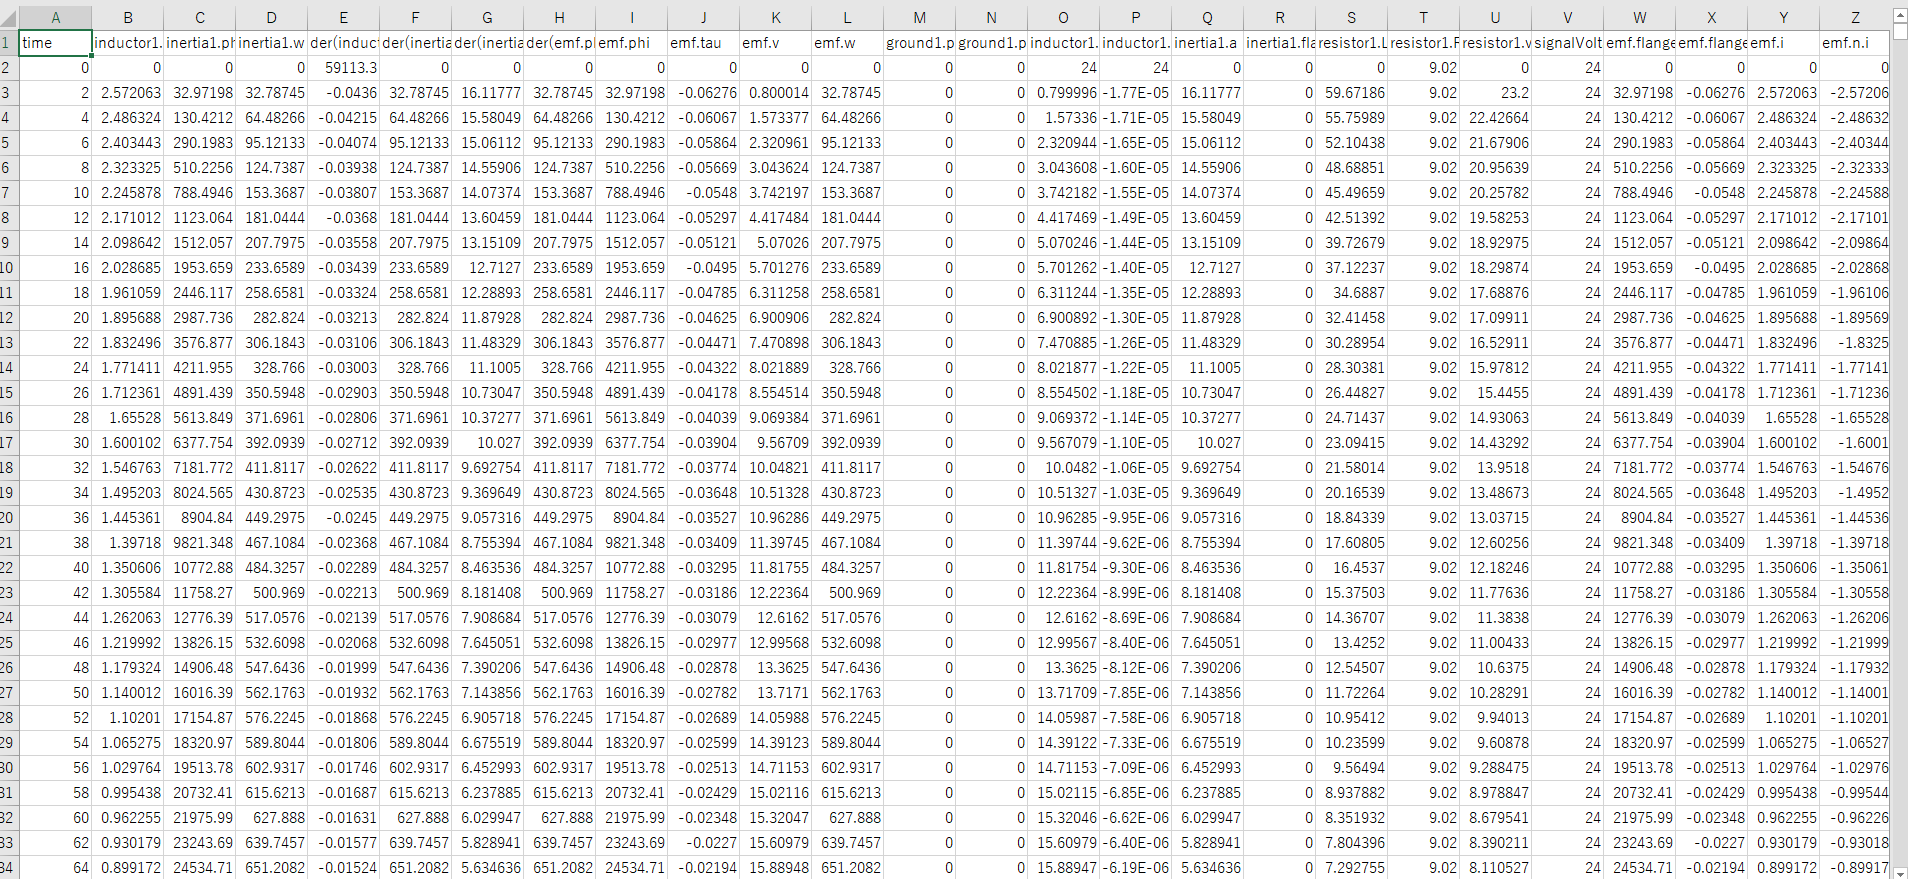
\includegraphics[width=16.5cm,height=10cm]{./Image/simyu_csv.png}
	\caption{図\ref{fig:tantai_model}のシミュレーション結果のcsvファイルの一部}
	\label{fig:simyu_csv}
\end{figure}

\begin{figure}[t]
	\centering
	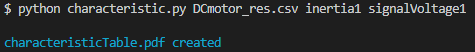
\includegraphics[width=12cm,height=1.5cm]{./Image/succes_comand.png}
	\caption{実行コマンド例}
	\label{fig:zikkou}
\end{figure}

% \clearpage
% \fboxsep=0pt
%  \fbox{
% 	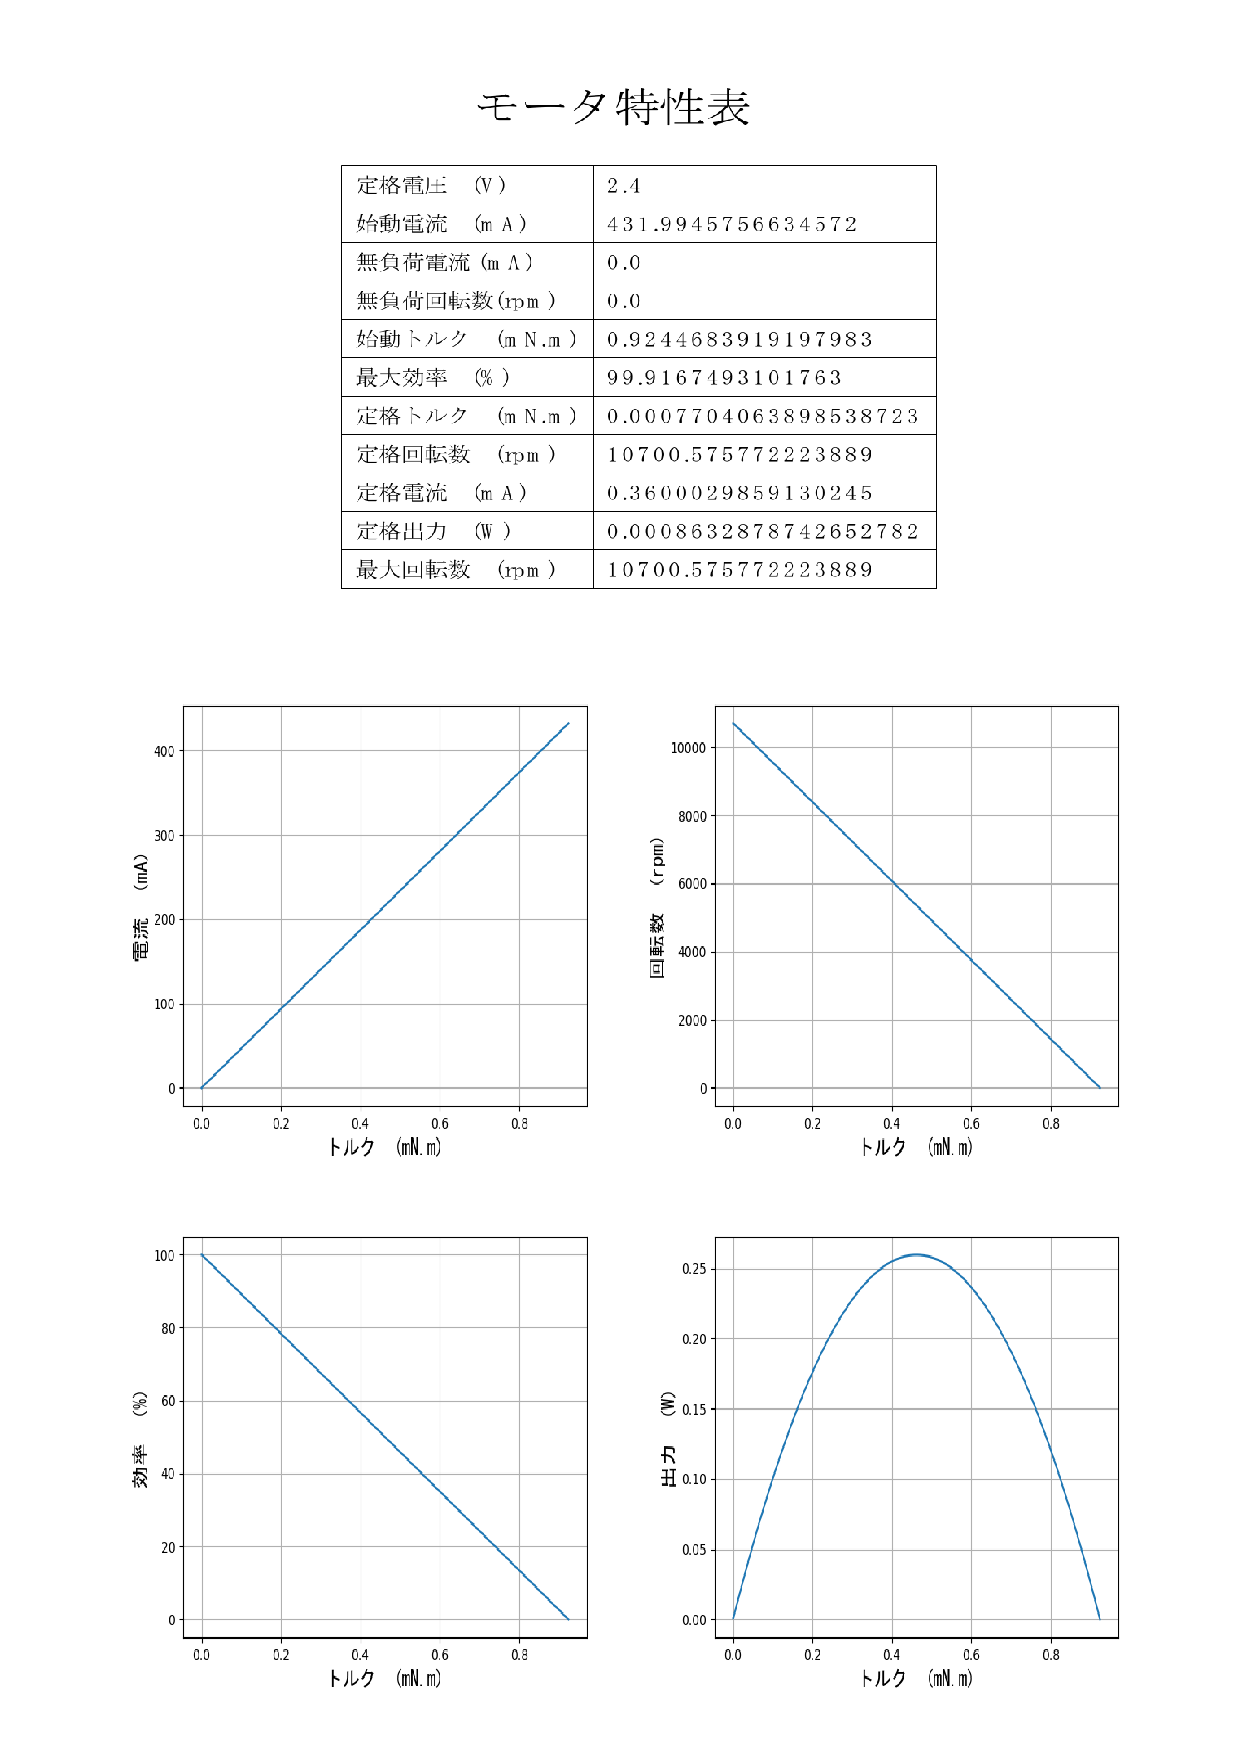
\includegraphics[width=16cm,pagebox=cropbox]{Image/characteristicTable.pdf} 
% 	% \label{fig:tokuseihyou}
%  }


\begin{figure}[t]
	\centering
	\fbox{
	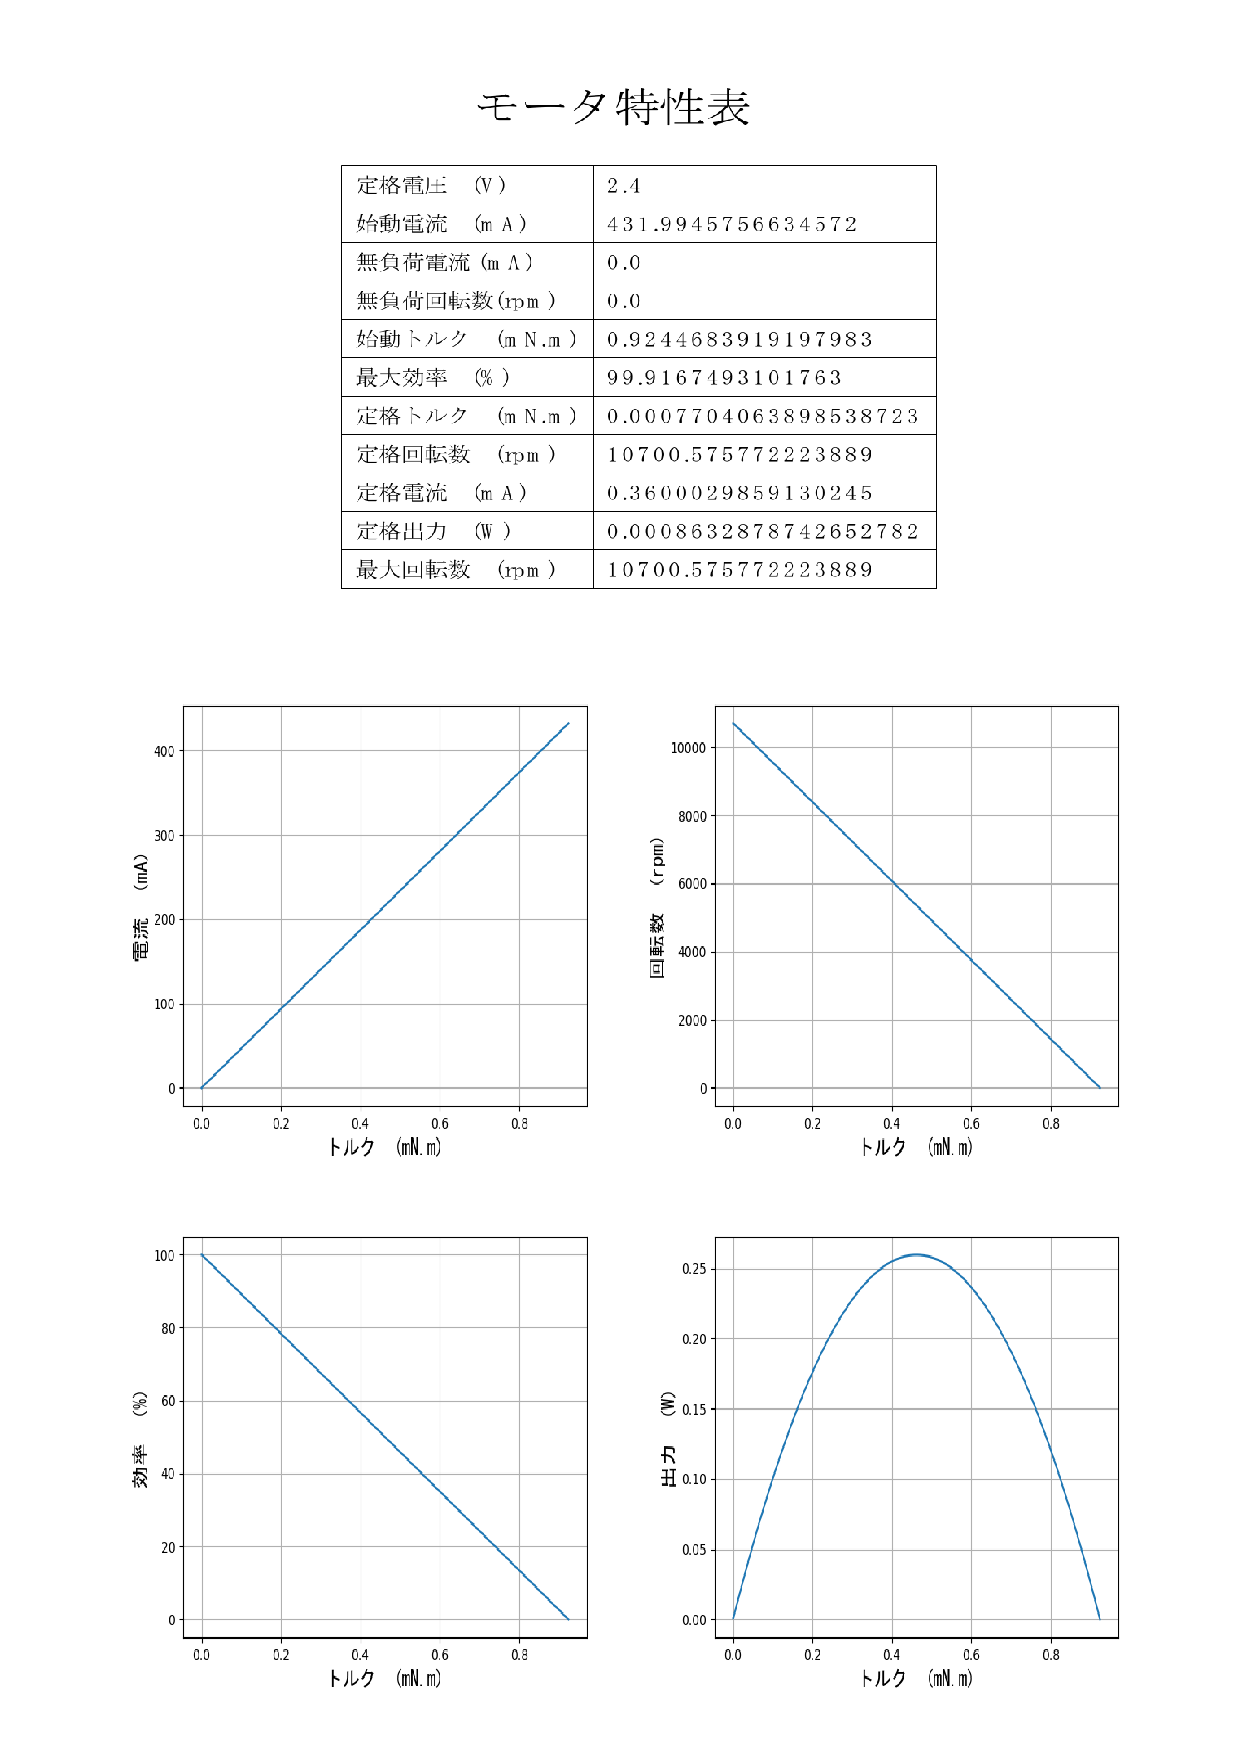
\includegraphics[width=16cm,pagebox=cropbox]{Image/characteristicTable.pdf} 
	}
	\caption{図\ref{fig:simyu_csv}のcsvファイルから作成したモータ特性表}
	\label{fig:tokuseihyou}
\end{figure}

\clearpage

% \subsection{実行コマンド}\label{sub:comand}

% \vspace{-5zh}

% \subsection{エラー表示}\label{sub:error}
\section{エラー表示}\label{error}
\ref{zikkou}節で、試作したツールを実行するためのコマンドは、「python characteristic.py 第1引数 第2引数 第3引数」であると述べた。
このコマンドを実行した際に、モータ特性表が作成できなかった場合、原因が2つ考えられ、それぞれの原因に即したエラー文を、画面上に表示する。\\
1つ目の原因は、第1引数で指定したcsvファイルのファイル名が間違っている場合が考えられ、エラー文として「ERROR : 指定したファイル名が間違っています」を、赤色で画面上に表示する。\\
例を、図\ref{fig:error_file}に示す。

2つ目の原因は、第2引数と第3引数のどちらか一方、もしくはその両方に間違いがあった場合が考えられ、エラー文として「ERROR : 指定したオブジェクト名が違います」を、赤色で画面上に表示する。\\
例を、図\ref{fig:error_comand}に示す。

\begin{figure}[t]
	\centering
	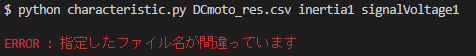
\includegraphics[width=12cm,height=1.5cm]{./Image/error_file.png}
	\caption{第1引数に誤りがあった場合のエラー文の例}
	\label{fig:error_file}
\end{figure}

\begin{figure}[t]
	\centering
	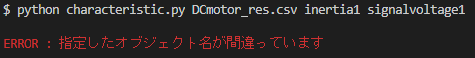
\includegraphics[width=12cm,height=1.5cm]{./Image/error_comand.png}
	\caption{第2、第3引数に誤りがあった場合のエラー文の例}
	\label{fig:error_comand}
\end{figure}